\documentclass[12pt]{opticajnl}
\journal{opticajournal} 

\setboolean{shortarticle}{true}


\usepackage{lineno}
\usepackage{setspace} % interlineado
\usepackage{tabularray}
\usepackage{multicol}

\usepackage{tikz}
\usepackage{xcolor}

\definecolor{crimson}{HTML}{ca3142}

%\linenumbers % Turn off line numbering for Optica Open preprint submissions.

\title{El Guachinche}

%\author[1,2,3]{Luis Ardévol Mesa, Carlos Martínez García \\ \copyrightstatement}
\author[1,2,3]{Luis Ardévol Mesa, Carlos Martínez García}

\begin{document}

\begin{titlepage}
\begin{center}
    \vspace*{5cm}
    
    {\huge\bfseries El Guachinche\par}
    \vspace{1cm}
    
    {\Large\color{crimson} Sistema de Inteligencia de Negocio\par}
    \vspace{1cm}
    
    
\begin{tikzpicture}
    \draw[thick, color=crimson] (0,0) -- (8,0);
    \end{tikzpicture}
    
    \vspace{1.5cm}
    {\large Luis Ardévol Mesa\\
    Carlos Martínez García\par}
    
    \vfill
    
    {\large Análisis y estrategias para\\
    la mejora del negocio\par}
    
    \vspace{2cm}
    
    {\large Diciembre, 2024\par}
\end{center}
\end{titlepage}

\maketitle

\section{Introducción}

\spacing{1.1}

Los \textit{guachinches} son establecimientos (en la propia vivienda del propietario) que surgen en la zona del norte del Tenerife como solución para vender el excedente de vino de cada cosecha. El vino se acompaña típicamente con platos tradicionales de la cocina canaria. Actualmente, según el Decreto 83/2013\footnote{\url{https://www.gobiernodecanarias.org/boc/2013/153/001.html}}, hay una regulación muy estricta amparando a estos locales y al viticultor; muchos establecimientos comúnmente denominados ``guachinches'', entran dentro de la categoría \textit{restaurante}, al salirse de lo establecido en este decreto. \\

El Guachinche nace de una idea sencilla pero atractiva: traer el espíritu de los tradicionales guachinches canarios al resto de España, pero con un toque especial. En nuestra cocina, las recetas isleñas comparten protagonismo con una cuidada selección de arepas para todos los públicos, todo esto acompañado de los mejores vinos de las Islas. Es ese equilibrio entre tradición y adaptación lo que nos hace únicos: cada local incorpora platos de la región, porque creemos que la gastronomía local es parte fundamental de nuestra historia. \\

No obstante, quien entra a El Guachinche no solo viene a comer. Para dar una experiencia lo más cercana posible y crear una atmósfera atractiva y familiar para los comensales, nuestros locales presentan una ambientación tradicional y hogareña. La experiencia no sería completa de no ser por nuestro personal, siempre cercano. \\

Actualmente, El Guachinche cuenta con 13 locales, repartidos en Canarias (7), Galicia (2), Andalucía (2) y Comunidad Valenciana (2). El crecimiento en los últimos dos años ha sido exponencial, por lo que desde la dirección de la empresa nos vemos en la necesidad de implementar un modelo de inteligencia de negocio que nos permita tomar decisiones basadas en datos, priorizando siempre al cliente. Algunos de los objetivos perseguidos serían la fidelización de clientes y la mejora de la experiencia general de los mismos, adaptar la oferta gastronómica a las preferencias de cada región o mantener un margen de beneficio cómodo en cada uno de los locales. \\


\subsection{Áreas de negocio}
Nuestra empresa se estructura en cinco áreas fundamentales, lo que nos permite abarcar todos los aspectos necesarios para mantener el correcto funcionamiento de los locales y asegurar su éxito a largo plazo:

\begin{itemize}
    \item \textbf{Área de gestión y finanzas:} Este área se preocupa por la rentabilidad del negocio, para lo cual es necesaria una gestión administrativa y financiera. Controla los costes, ingresos y presupuesto, además de establecer estrategias para optimizar la rentabilidad de cada local.
    \item \textbf{Área de expansión:} La apertura de un nuevo local nunca es tarea fácil. Para ello, disponemos del área de expansión, que estudia el mercado en busca de nuevas oportunidades de crecimiento en ubicaciones aún no exploradas por El Guachinche.
    \item \textbf{Área de gestión de clientes:} Nuestra prioridad es la satisfacción del cliente. Este área se ocupa de garantizar la mejor experiencia posible en cada uno de nuestros establecimientos.
    \item \textbf{Área de producción y operaciones:} Gestionar suministros de calidad en todos nuestros locales es una tarea complicada. El área de producción y operaciones se encarga de coordinar la cadena de suministro, tanto de productos canarios como locales. Esto permite mantener unos estándares de calidad y controlar el \textit{stock}.
    \item \textbf{Área comercial:} Desarrolla las estrategias de mercado, adaptando precios y promociones a cada zona mientras mantiene la coherencia de marca en todos los establecimientos.
\end{itemize}













\section{Objetivos de negocio}

\subsection{Área de gestión y finanzas}

\subsubsection*{CSF1: Garantizar la rentabilidad de cada local.}

La rentabilidad de los locales es uno de los objetivos más importantes de cualquier negocio. A través de la gestión minuciosa de los ingresos y los costos operativos, podemos asegurar que cada local mantenga un rendimiento económico sostenible, lo que garantizará parte del éxito financiero de la cadena. Para lograr este objetivo, se utilizan los siguientes indicadores:

\begin{itemize}
    \item \textbf{PI1.1: Fijar margen de beneficio bruto en un 70\%.} Este indicador mide los beneficios obtenidos tras considerar los costes directos asociados. El objetivo será que cada local fije este margen en torno a un 65-70\%, lo que aseguraría cubrir los gastos del local y permitiría un margen de beneficio neto del 10-15\%. 
    \item \textbf{PI1.2: Disminuir coste operativo por local en un 10\%.} Dentro de estos costes se incluyen el alquiler, el salario del personal, los suministros y gastos extra, como luz, agua, limpieza, mantenimiento, etc. La meta es reducir estos gastos en un 10\% en cada local sin comprometer la calidad del servicio, lo que permitirá aumentar la rentabilidad.
    \item \textbf{PI1.3: Aumentar el promedio de gasto por cliente en un 5\%.} Este indicador mide los ingresos promedio generados por cada cliente. El objetivo sería aumentarlo sin elevar siginificativamente el coste de cada plato, lo que indicaría un mayor consumo por cliente. 
    \item \textbf{PI1.4: Fijar tasa de ocupación del local en un 80\%.} Para asegurar la rentabilidad de cada local, es crucial aprovechar de forma eficiente el espacio durante el servicio. Mantener un alto porcentaje de las mesas disponibles ocupadas es un indicador clave de la rentabilidad del local.
    \item \textbf{PI1.5: Reducir porcentaje de desperdicio de alimentos a un 2\%.} El desperdicio de alimentos es inaceptable en nuestros locales, no solo por las consecuencias económicas. Se exige mantenerlo por debajo del 2\% para asegurar la rentabilidad de los productos. 
\end{itemize}






\subsection{Área de expansión}

\subsubsection*{CSF2: Mantener un crecimiento escalado y sostenible.}

Mantener la esencia del negocio es de vital importancia. Por ello, queremos garantizar que un crecimiento de la cadena sostenible, que no comprometa la calidad del servicio y la experiencia del cliente. Para cumplir este objetivo, fijamos los siguientes indicadores:

\begin{itemize}
    \item \textbf{PI2.1: Bajo número de nuevos locales abiertos anualmente.} Una vez establecido el negocio, no existe una necesidad de expansión rápida y descontrolada. El número de nuevos locales abiertos cada año será de máximo 3. Esto garantiza una correcta gestión de las finanzas y la logística de los mismos, haciendo que, al abrir nuevos locales, los ya establecidos se encuentren en una situación financiera estable.
    \item \textbf{PI2.2: Reducir tiempo promedio de rentabilidad de nuevos locales.} Este indicador va de la mano con el anterior. Reducir el tiempo que un nuevo local tarda en ser rentable a menos de 12 meses hace posible la apertura anual de nuevos locales sin aumentar en exceso la logística.
    \item \textbf{PI2.3: Incremento en ingresos totales del 15\%.} Buscamos un crecimiento sostenido del negocio. Por ello, un crecimiento anual del 10-15\% resulta adecuado.
    \item \textbf{PI2.4: Tasa de éxito de nuevos locales de un 90\%.} El éxito de los nuevos locales se mide en base a la satisfacción de sus clientes y el alcance de objetivos (como la rentabilidad del primer año). Así, buscamos fijar la tasa de éxito de los nuevos locales en no menos de un 90\%.  
\end{itemize}






\subsection{Área de gestión de clientes}

\subsubsection*{CSF3: Maximizar la satisfacción y fidelización del cliente.}

El cliente es el centro de la estrategia de El Guachinche. Aumentar la satisfacción del cliente y fomentar la fidelización es esencial para el éxito a largo plazo de la cadena. A través de la atención personalizada y la calidad y cercanía del servicio, se busca crear una experiencia única para el cliente. Los indicadores clave en este área son:

\begin{itemize}
    \item \textbf{PI3.1: Valoración de satisfacción del cliente de $4.5$.} Nuestros locales realizan encuestas de satisfacción recurrentes a sus clientes, con el fin de obtener \textit{feedback} acerca de la calidad de la comida, el servicio y el ambiente del local. Mantener una satisfacción por encima del $4.5/5$ en estas encuestas es un objetivo principal para el éxito de la cadena.
    \item \textbf{PI3.2: Aumentar la recuencia de visitas por cliente.} El objetivo es que nuestros clientes habituales visiten el local al menos 2 veces al mes. Esto indica un nivel de satisfacción adecuado y permite apoyar la economía del local en una clientela ya estable.
    \item \textbf{PI3.3: 90\% de quejas resueltas satisfactoriamente.} Si bien no es deseable contar con un gran número de quejas, estas forman parte de un negocio. En este aspecto, el objetivo es resolver de forma satisfactoria al menos un 90\% de las mismas, lo que ayudará a mejorar la imagen de cara al público y la retención de clientes.
    \item \textbf{PI3.4: Aumentar los clientes nuevos por recomendación.} No hay mejor publicidad que la proporcionada por el propio cliente boca a boca. Este método, además, se alinea a la perfección con la filosofía tradicional de nuestra cadena. En cuanto a la captación de nuevos clientes, el objetivo sería que al menos un 80\% de los nuevos clientes vengan por recomendación, lo que indicaría que los clientes actuales están promocionando de forma activa el negocio.
\end{itemize}

\subsection{Área de producción y operaciones}

\textbf{CSF4: Eficiencia en la gestión de la cadena de suministro.}

La cadena de suministro es crucial para garantizar que los productos estén siempre disponibles, frescos y de la mejor calidad. Un manejo eficiente del inventario, logística y reposición de productos es vital para evitar rupturas de \textit{stock} y sobrecostos. Como indicadores clave en este área se plantean los siguientes:

\begin{itemize}
    \item \textbf{PI4.1: Tiempo de reposición de productos menor a 48 horas.} Con esto se hace referencia al tiempo trancurrido entre un pedido y la entrega del mismo en el local. Para que estos últimos dispongan de productos frescos y disponibles, debemos asegurar que este tiempo de reposición sea de 24 horas para productos locales y menor a 48 horas para los productos que vengan desde Canarias. 
    \item \textbf{PI4.2: Nivel de inventario crítico por debajo del 5\%.} El inventario crítico hace referencia a aquellos productos que, por su poca cantidad disponible, están en riegso de ruptura. Para disponer siempre de suficiente inventario para el día a día, buscamos fijar el nivel de inventario crítico en menos de un 5\%. No obstante, se busca un compromiso para evitar el exceso de \textit{stock} (lo que ayuda a reducir el desperdicio de alimentos).
    \item \textbf{PI4.3: Reducir el coste logístico por pedido en un 10\%.} Para reducir los costes asociados a cada pedido de suministros, se busca depender todo lo posible de productos de kilómetro 0. El objetivo final es reducir los costes actuales en un 5-10\%.
\end{itemize}

\textbf{CSF5: Flexibilidad operativa.}

En unos locales con la demanda que presenta El Guachinche, es necesario mantener cierta flexibilidad operativa que permita resolver problemas inesperados de forma que afecte lo mínimo posible al cliente. Para mejorar nuestra capacidad de ajuste a la demanda y condiciones del mercado, definimos los siguientes indicadores:

\begin{itemize}
    \item \textbf{PI5.1: Menú adaptable de forma parcial.} Buscamos que al menos un 15\% de la carta de cada local sea variable en función de la estacionalidad de los productos. 
    \item \textbf{PI5.2: Disponibilidad de 2 proveedores alternativos.} Para evitar cortes de suministros y poder disponer siempre de productos frescos en los locales, resulta necesario que cada local tenga al menos dos proveedores de calidad para momentos críticos.
    \item \textbf{PI5.3: Tiempo de parada por falta de suministro, 0.} Con la adapatabilidad del menú y la exigencia de proveedores alternativos, buscamos que no haya cortes o reducciones en las horas de servicios de cada local.    
\end{itemize}





\subsection{Área comercial}

\subsubsection*{CSF6: Coherencia de la marca.}

Como se puede intuir por la descripción e idea del negocio, buscamos una imagen de marca reconocible y coherente con los valores que representamos. Al ser una cadena nacional, la coherencia cobra un papel de gran relevancia. Para garantizar esta última, fijamos los siguientes indicadores:

\begin{itemize}
    \item \textbf{PI6.1: Cumplimiento de estándares de marca en todos los locales.} El 100\% de los locales deben cumplir con las directrices de imagen y servicio fijadas por la directiva de forma transversal.
    \item \textbf{PI6.2: Comunicación y publicidad consistentes.} Las campañas de publicidad de cada local deben estar alineadas con los valores que representa la empresa. El Guachinche se debe ver como un todo y no como locales individuales.
    \item \textbf{PI6.3: Formación del 100\% del personal.} Todo el personal debe comprender los valores que representa la cadena y conocer la cultura y tradición local. En este sentido, el 100\% de los trabajadores deberá recibir cierta formación.
\end{itemize}

A continuación, se incluye una tabla a modo de síntesis de los factores críticos de éxito y los indicadores clave de rendimiento que se han explicado:


\begin{longtblr}[caption = {Síntesis factores críticos de éxito con tipo de indicador y acción},]{colspec = {p{1.75cm}p{2.5cm}Xp{1.9cm}p{1.5cm}X}, rowhead = 1,}
\hline\hline
\textbf{Factor Crítico de Éxito (CSF)} & \textbf{Identificador de indicador} & \textbf{Indicador} & \textbf{Tipo de indicador} & \textbf{Meta} & \textbf{Acción} \\ \hline\hline
CSF1 & PI1.1 & Aumentar margen de beneficio bruto & \textit{Lagging} & 65-70\% & Revisar precios y optimizar costes. \\ \hline
CSF1 & PI1.2 & Reducir coste operativo por local & \textit{Lagging} & $-10$\% & Negociar contratos y mejorar eficiencia operativa. \\ \hline
CSF1 & PI1.3 & Aumentar gasto por cliente & \textit{Lagging} & +5-10\% & Introducir ofertas atractivas y mejorar el menú. \\ \hline
CSF1 & PI1.4 & Aumentar tasa de ocupación & \textit{Lagging} & 75-80\% & Promociones en horarios de baja demanda. \\ \hline
CSF1 & PI1.5 & Reducir desperdicio de alimentos & \textit{Lagging} & $<2$\% & Implementar control estricto de inventario. \\ \hline\hline
CSF2 & PI2.1 & Pocos nuevos locales por año & \textit{Leading} & $\leq 3$ & Planificar aperturas estratégicas anuales. \\ \hline
CSF2 & PI2.2 & Reducir tiempo de rentabilidad de nuevos locales & \textit{Lagging} & $< 12$ meses & Supervisar rendimiento inicial y ajustar estrategias. \\ \hline
CSF2 & PI2.3 & Aumento de ingresos totales & \textit{Lagging} & $+15$\% & Incrementar promociones y optimizar márgenes. \\ \hline
CSF2 & PI2.4 & Fijar tasa de éxito de nuevos locales & \textit{Lagging} & $\geq 90$\% & Garantizar formación adecuada y consistencia operativa. \\ \hline\hline
CSF3 & PI3.1 & Fijar valoración de satisfacción del cliente & \textit{Lagging} & $\geq 4.5$ & Realizar encuestas de satisfacción y actuar según el feedback. \\ \hline
CSF3 & PI3.2 & Aumentar recurrencia de visitas & \textit{Lagging} & $\geq 2$/mes & Crear programas de fidelización. \\ \hline
CSF3 & PI3.3 & Fijar quejas resueltas satisfactoriamente & \textit{Lagging} & 90\% & Mejorar tiempos de respuesta y procesos de resolución. \\ \hline
CSF3 & PI3.4 & Aumentar nuevos clientes por recomendación & \textit{Leading} & $\geq 80$\% & Incentivar recomendaciones mediante beneficios exclusivos. \\ \hline\hline
CSF4 & PI4.1 & Fijar tiempo de reposición de productos & \textit{Lagging} & $< 48$h & Optimizar logística y establecer acuerdos con proveedores locales. \\ \hline
CSF4 & PI4.2 & Reducir nivel de inventario crítico & \textit{Lagging} & $< 5$\% & Monitorear inventarios en tiempo real. \\ \hline
CSF4 & PI4.3 & Reducir costes logísticos por pedido & \textit{Lagging} & $-10$\% & Consolidar pedidos y negociar tarifas de transporte. \\ \hline\hline
CSF5 & PI5.1 & Adaptabilidad del menú & \textit{Leading} & 15\% & Introducir platos de temporada o adaptados regionalmente. \\ \hline
CSF5 & PI5.2 & Tener proveedores alternativos & \textit{Leading} & 2 & Auditar y registrar opciones de suministro secundarias. \\ \hline
CSF5 & PI5.3 & Reducir el tiempo de parada por falta de suministros & \textit{Lagging} & 0 & Establecer sistemas de alerta para reposición temprana. \\ \hline\hline
CSF6 & PI6.1 & Cumplimiento de estándares de la marca por los locales & \textit{Leading} & 100\% & Auditorías regulares de calidad en todos los locales. \\ \hline
CSF6 & PI6.2 & \textit{Marketing} consistente & \textit{Leading} & Campaña uniforme & Supervisar las campañas publicitarias regionales. \\ \hline
CSF6 & PI6.3 & Formar al personal en cultura y tradición local & \textit{Leading} & 100\% del personal & Desarrollar y ejecutar programas de formación continua. \\ \hline\hline
\end{longtblr}


\section{Diseño lógico}

\subsection{Procesos de negocio}

A continuación, identificamos los principales procesos de negocio de El Guachinche, junto con el hecho que representa cada uno. Nos centraremos en los 3 principales, que son los que más impacto tienen en la compañía (y los que aportan un mayor número de dimensiones). Los principales procesos de negocio identificados son los siguientes:


\subsubsection{Gestión financiera (proceso 1)}

Para garantizar la rentabilidad de cada local, es necesario llevar un control de los gastos e ingresos de cada uno de ellos, así como el número de clientes que recibe. Con este proceso nos aseguramos de recopilar la información económica de cada local y concluir el rendimiento de cada uno. Este proceso queda definido por las siguientes características:
\begin{itemize}
\item \textbf{Granularidad:} Mensual.
\item \textbf{Tasa de refresco:} Mensual.
\item \textbf{Tipo de tabla de hecho:} Hecho acumulativo.
\item \textbf{Medidas:} coste, ingresos, clientes y nuevos clientes.
\begin{itemize}
\item coste; medida aditiva: recoge los gastos de cada local durante ese mes. Se obtiene como la suma del alquiler, el salario del personal, los suministros y gastos extra, como luz, agua, limpieza, mantenimiento, etc. 
\item ingresos; medida aditiva: recoge los ingresos de cada local durante ese mes. Se obtiene como la suma de los ingresos por vía presencial y a domicilio.
\item clientes; medida aditiva: recoge el número total de clientes que han visitado el local durante ese mes. Se obtiene a partir de los datos proporcionados por cada local.
\item nuevos\_clientes; medida aditiva: recoge el número de clientes nuevos que han visitado el local durante ese mes. Aunque este número está incluido en el total de clientes, se recoge por separado para poder sacar estadísticas de interés en relación al crecimiento de la clientela, entre otras. Se obtiene a partir de los datos proporcionados por cada local.
\end{itemize}
\end{itemize}

\begin{figure}[h]
\centering
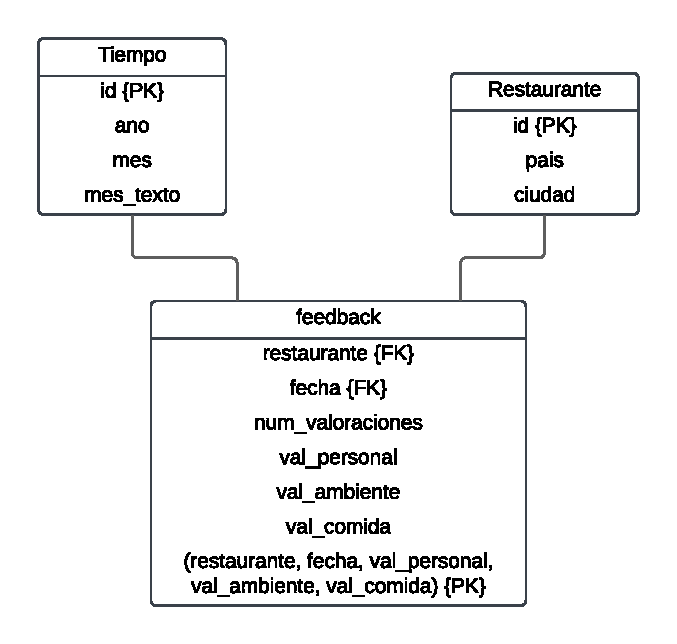
\includegraphics[width=0.6\textwidth]{fotos/fin.pdf}
\caption{Esquema conceptual del proceso 1.}
\label{fig:esquema_proceso1}
\end{figure}

\subsubsection{Gestión de ventas e inventario (proceso 2)}

Estudiada la rentabilidad de cada local, nos gustaría también conocer el desglose de ventas de cada uno de los locales. Esto permite un análisis exhaustivo de la actividad de cada local y ayuda a identificar los productos que deben presentar mayor disponibilidad en el inventario. Este proceso queda definido por las siguientes características (está estrechamente relacionado con la dimensión ``productos'', que contendrá información sobre la oferta de platos y sus precios):
\begin{itemize}
\item \textbf{Granularidad:} Mensual.
\item \textbf{Tasa de refresco:} Semanal.
\item \textbf{Tipo de tabla de hecho:} Hecho acumulativo.
\item \textbf{Medidas:} número de ventas de cada platos e ingresos de los mismos.
\begin{itemize}
\item num\_ventas; medida aditiva: recoge el número de ventas de cada plato durante ese mes. Se obtiene a partir de los datos proporcionados por cada local de forma semanal, y se acumulan los datos de cada mes.
\item ingresos; medida calculada: recoge los ingresos generados por cada plato durante ese mes. Se obtiene como el producto del número de ventas de un plato por su precio (en la dimensión ``productos'').
\end{itemize}
\end{itemize}

\begin{figure}[h]
\centering
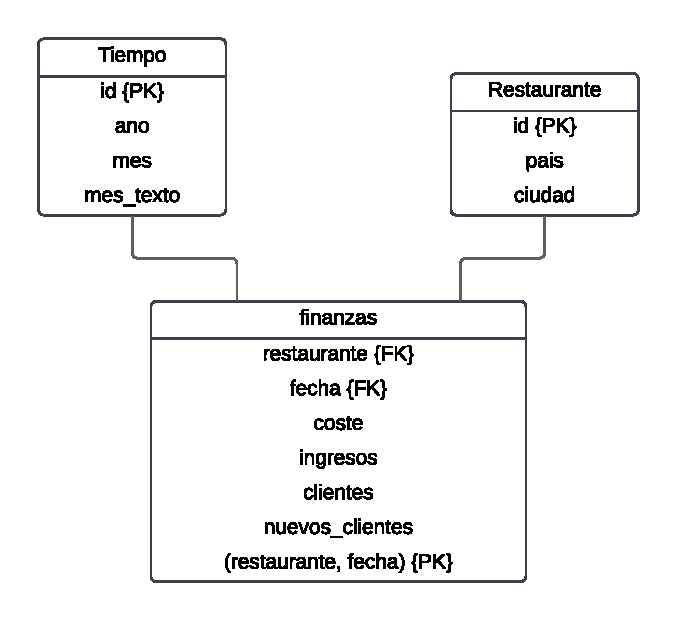
\includegraphics[width=0.6\textwidth]{fotos/prods.pdf}
\caption{Esquema conceptual del proceso 2.}
\label{fig:esquema_proceso2}
\end{figure}

\subsubsection{Gestión de clientes (proceso 3)}

Como hemos comentado anteriormente, el cliente es nuestra prioridad. Por ello, necesitamos llevar un control de la satisfacción de los mismos con cada local. Esta satisfacción la desglosamos en 3 aspectos fundamentales: la calidad de la comida, el ambiente del local y la atención del personal. Este proceso queda definido por las siguientes características:
\begin{itemize}
\item \textbf{Granularidad:} Mensual.
\item \textbf{Tasa de refresco:} Diaria.
\item \textbf{Tipo de tabla de hecho:} Hecho acumulativo.
\item \textbf{Medidas:} valoración del personal, valoración del ambiente y valoración de la comida. Todas estas medidas se obtiene a partir de los datos proporcionados por cada local diariamente, y se acumulan los datos de cada mes
\begin{itemize}
\item num\_valoraciones
\item valoracion\_personal: satisfacción (de 0.0 a 5.0) con el servicio prestado por el personal.
\item valoracion\_ambiente: satisfacción (de 0.0 a 5.0) con el ambiente del local.
\item valoracion\_comida: satisfacción (de 0.0 a 5.0) con la calidad de la comida.
\end{itemize}
\end{itemize}

\begin{figure}[H]
\centering
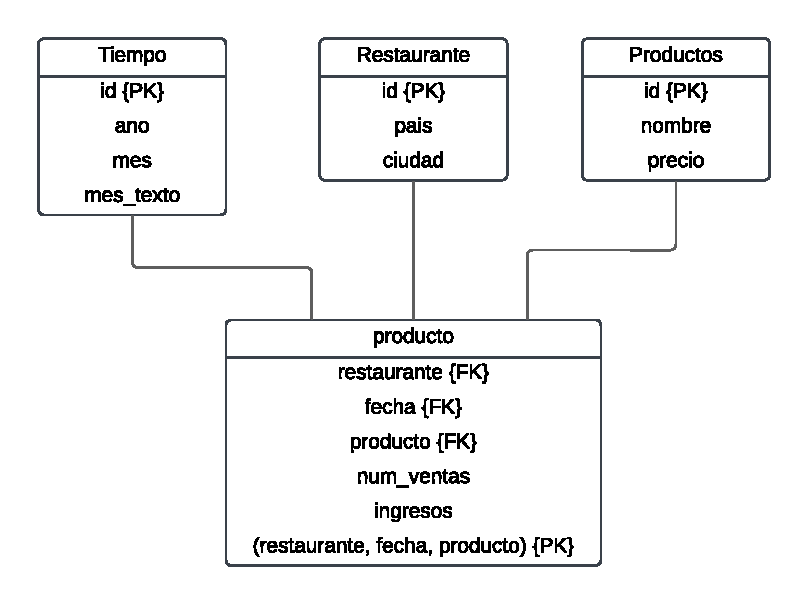
\includegraphics[width=0.6\textwidth]{fotos/feed.pdf}
\caption{Esquema conceptual del proceso 3.}
\label{fig:esquema_proceso3}
\end{figure}

Para finalizar, mostramos un esquema reducido general de los tres procesos a implementar en la figura \ref{fig:esquema_almacen}

\begin{figure}[H]
\centering
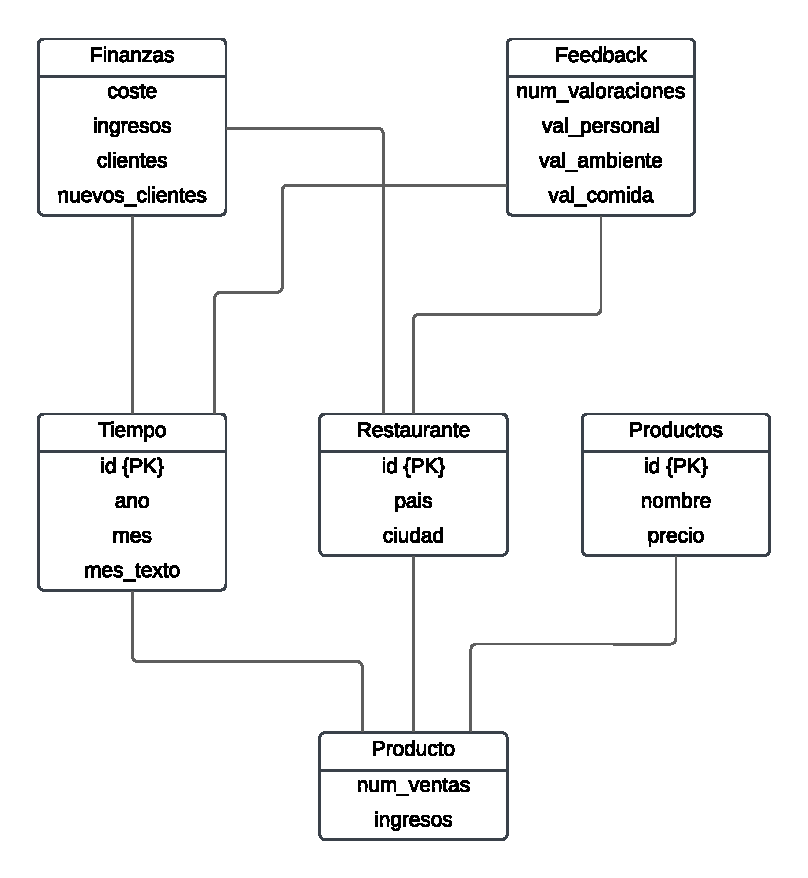
\includegraphics[width=0.6\textwidth]{fotos/3.pdf}
\caption{Esquema conceptual del almacén de datos.}
\label{fig:esquema_almacen}
\end{figure}


\subsection{Dimensiones}

Las dimensiones seleccionadas para representar correctamente los procesos anteriores son las siguientes (mostradas de forma adelantada en la figura \ref{fig:esquema_almacen}, así como en las figuras \ref{fig:esquema_proceso1}, \ref{fig:esquema_proceso2} y \ref{fig:esquema_proceso3}):
\begin{itemize}
\item \textbf{Tiempo}: esta dimensión almacena la fecha de los datos que son agregados a las tablas de hechos, en formato YYYY-MM. La dimensión temporal de los datos se representa mediante una jerarquía de dos niveles: año y mes. Esta es un dimensión compartida entre los tres hechos antes mencionados y tiene los siguientes atributos:
\begin{itemize}
\item id. Esta es la clave primaria, un serial de tipo \texttt{Integer} que se genera automáticamente cada vez que se inserta un nuevo mes.
\item ano. Este atributo es de tipo \texttt{Integer} y representa el año.
\item mes. Este atributo es de tipo \texttt{Integer} y representa el mes dentro del año.
\item mes\_texto. Este atributo es de tipo \texttt{String} y representa el nombre del mes correspondiente.
\end{itemize}
\item \textbf{Restaurante}: la dimensión restaurante actúa como dimensión geográfica. Se tendrán en cuenta todos los locales de la cadena y constituirá una jerarquía de dos niveles, uno para el país y otro para la ciudad. Esta dimensión, de nuevo, es compartida por los tres hechos ya mencionados, y tiene los siguientes atributos:
\begin{itemize}
\item id. Esta es la clave primaria, un serial de tipo \texttt{Integer} que se genera automáticamente cada vez que se inserta un nuevo local.
\item pais. Este atributo es de tipo \texttt{String} y representa el país en el que se encuentra el local.
\item ciudad. Este atributo es de tipo \texttt{String} y representa la ciudad en la que se encuentra el local.
\end{itemize}
\item \textbf{Producto}: la dimensión producto recoge todos los platos ofertados en los locales de la cadena. Esta es una dimensión plana que muestra los productos y el precio asociado a cada uno de ellos. Esta dimensión es exclusiva del proceso 2, y tiene los siguientes atributos:
\begin{itemize}
\item id. Esta es la clave primaria, un serial de tipo \texttt{Integer} que se genera automáticamente cada vez que se inserta un nuevo producto (plato, bebida, etc).
\item nombre. Este atributo es de tipo \texttt{String} y representa el nombre del producto.
\item precio. Este atributo es de tipo \texttt{Numeric} y representa el precio del producto.
\end{itemize}
Los precios de los platos en cada local son relativamente estáticos, pero como cualquier otro producto, pueden cambiar con el tiempo. Por ello, esto es una dimensión lentamente cambiante, donde el precio es susceptible a cambio. La solución propuesta para manejar esto es crear un nuevo registro en la dimensión
\end{itemize}


\subsection{Cálculo de los indicadores a partir del diseño lógico}

En el apartado 2 identificamos numerosos procesos e indicadores. Por simplicidad, reduciremos la descripción del cálculo de los indicadores a los relaciones estrechamente con los hechos y dimensiones antes mencionados. Concretamente, trateremos los indicadores asociados al CSF1 (garantizar la rentabilidad de cada local), CSF3 (maximizar la satisfacción y fidelización del cliente) y CSF4 (eficiencia en la gestión de la cadena de suministro). El cálculo de los indicadores asociados a estos factores críticos de éxito es el siguiente:

\begin{longtblr}[caption = {Cálculo de indicadores asociados a procesos modelados (con un $^*$ indicamos procesos para los que aún no se disponen de las medidas necesarias, que deben proporcionar los locales). Aquí, usaremos el subíndice $i$ para hacer referencia al mes, por lo que, por ejemplo, $i-1$, será una magnitud asociada al mes anterior (considerando la granularidad mensual que estamos usando)},]{colspec = {p{2.5cm}Xp{2cm}X}, rowhead = 1,}
\hline\hline
\textbf{Identificador de indicador} & \textbf{Indicador} & \textbf{Proceso de negocio} & \textbf{Descripción del cálculo} \\ \hline\hline
PI1.1 & Aumentar margen de beneficio bruto & Proceso 1 & $\text{ingresos}_i - \text{ingresos}_{i-1}$  \\ \hline
PI1.2 & Reducir coste operativo por local & Proceso 1 & $\text{coste}_i - \text{coste}_{i-1}$ \\ \hline
PI1.3 & Aumentar gasto por cliente & Proceso 1 & $\displaystyle\frac{\text{ingresos}_i}{\text{clientes}_i}$ \\ \hline
PI1.4 & Aumentar tasa de ocupación & Proceso 1 & $\displaystyle\frac{\text{clientes}_i}{\text{capacidad\_max} \times \text{num\_turnos}}$ \\ \hline
PI1.5 & Reducir desperdicio de alimentos $^*$ & Proceso 1 & $\displaystyle\frac{\text{peso\_alimentos\_desperdiciados}_i}{\text{peso\_alimentos\_inventario}_i}$ \\ \hline\hline
PI3.1 & Fijar valoración de satisfacción del cliente & Proceso 2 &  \\ \hline
PI3.2 & Aumentar recurrencia de visitas & Proceso 2 &  \\ \hline
PI3.3 & Fijar quejas resueltas satisfactoriamente & Proceso 2 &  \\ \hline
PI3.4 & Aumentar nuevos clientes por recomendación & Proceso 2 &  \\ \hline\hline
PI4.1 & Fijar tiempo de reposición de productos & Proceso 3 &  \\ \hline
PI4.2 & Reducir nivel de inventario crítico & Proceso 3 &  \\ \hline
PI4.3 & Reducir costes logísticos por pedido & Proceso 3 &  \\ \hline\hline
\end{longtblr}

Algunas requieren explicación adicional, ya que implican medidas no consideradas anteriormente. En el cálculo de la tasa de ocupación, se menciona $\text{capacidad\_max}$ y $\text{num\_turnos}$. Estos valores son (en principio) fijos para cada restaurante: el primero nos da la capacidad máxima de la sala, y el segundo el número de turnos ese mes, que deberían ser unos 48 (2 por día, 6 días por semana).

\end{document}